% !Tex root = main.tex
\section{Introduction}

\begin{figure}[h]
  \begin{center}
    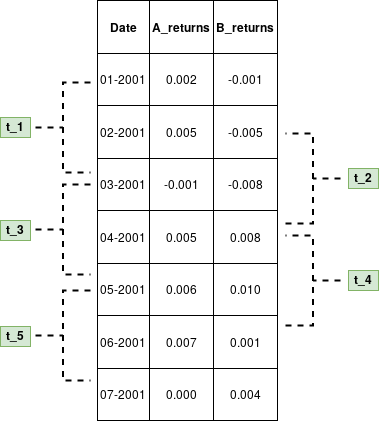
\includegraphics[width=.50\textwidth]{images/rolling_window.png}
    \caption{Illustration of the rolling-window approach for a time-series containing seven time-steps filled with mock-data. Five subsets of length 3 divide the time-series.}
    \label{fig:rolling_window}
  \end{center}
\end{figure}
This approach is schematically described in figure \ref{fig:rolling_window}.\\

